\documentclass[11pt,a4paper]{article}
\usepackage[utf8]{inputenc}
\usepackage[T1]{fontenc}
\usepackage[french]{babel}
\usepackage[margin=2cm]{geometry}
\usepackage{graphicx}
\usepackage{hyperref}
\usepackage{enumitem}
\usepackage{xcolor}
\usepackage{titlesec}

\setlist{nosep,leftmargin=1.2em}
\titlespacing*{\section}{0pt}{0.6em}{0.3em}
\titlespacing*{\subsection}{0pt}{0.4em}{0.2em}
\titleformat{\section}{\normalfont\bfseries\large}{\thesection}{0.5em}{}
\titleformat{\subsection}{\normalfont\bfseries}{\thesubsection}{0.5em}{}
\setlength{\parskip}{0.3em}
\setlength{\parindent}{0pt}

\title{\vspace{-1.5cm}Rapport individuel --- It\'eration 1}
\author{Alexis Briend (\texttt{abd7852}) --- Projet Long SHDL}
\date{13 avril 2026}

\begin{document}
\maketitle
\vspace{-1.5em}

\section*{Contexte et objectif de l'it\'eration}

Le projet consiste \`a d\'evelopper un simulateur de circuits logiques d\'ecrits en langage SHDL, avec une interface JavaFX. L'\'equipe compte neuf personnes r\'eparties sur six axes (\'editeur, parser, automates, simulateur, IHM, int\'egration). Ma responsabilit\'e porte sur la structure g\'en\'erale de l'application et sur l'\textbf{interpr\'etation du SHDL} (ticket \textsc{Scrum-23}). L'objectif de l'it\'eration 1 \'etait de poser les fondations techniques~: arborescence, gestion de d\'ependances, grammaire SHDL et parser vers un AST exploitable par les modules aval.

\section*{Activit\'es r\'ealis\'ees}

\begin{itemize}
  \item \textbf{Squelette JavaFX/Gradle} sous \texttt{src/main/java/fr/n7/shdl/} (packages \texttt{model}, \texttt{view}, \texttt{controller}), avec \texttt{module-info} et \texttt{build.gradle}.
  \item \textbf{Grammaire SHDL LL(1)} formalis\'ee dans \texttt{parser/ll1/grammar/}~: grammaire d\'eclarative (r\`egles comme objets Java), calcul de \textsc{First}/\textsc{Follow}, v\'erificateur automatique de conflits LL(1).
  \item \textbf{AST immuable} (\texttt{parser/ll1/ast/})~: hi\'erarchie \texttt{Node} $\to$ \texttt{Expression}/\texttt{Statement}, champs \texttt{final}, collections copi\'ees via \texttt{List.copyOf}, non-null garanti, Visitor typ\'e \texttt{<R>}.
  \item \textbf{Parseur \`a descente r\'ecursive} avec lookahead 2 sur les instances, messages d'erreur contextuels et enrichis (code + position + attendu).
  \item \textbf{Documentation}~: sp\'ecification \texttt{docs/specs/}, plan d'ex\'ecution \texttt{docs/plans/}, bilan d'it\'eration \texttt{docs/sprint1/}.
\end{itemize}

\section*{R\'esultats}

\begin{itemize}
  \item \textbf{107 tests JUnit verts} r\'epartis sur 23 classes (grammaire, tokens, AST, visiteur par d\'efaut, invariants runtime, cas n\'egatifs, bout-en-bout sur \texttt{ET}, \texttt{BasculeD}, \texttt{FsmSync}, \texttt{DecBCD}).
  \item \textbf{39 fichiers Java} produits sous \texttt{parser/ll1/}.
  \item Une \textbf{limite connue} documente un pi\`ege grammatical (\texttt{TERM\_REST}, wildcard FSM suivi d'un STAR de r\`egle voisine). Un test n\'egatif la rend visible, la correction est report\'ee \`a l'it\'eration 2.
  \item Une revue critique interne a fait \'emerger cinq d\'efauts (traversal incomplet du \texttt{DefaultVisitor}, champs redondants, invariants manquants), tous corrig\'es dans la branche avant la fin du sprint.
\end{itemize}

\begin{center}
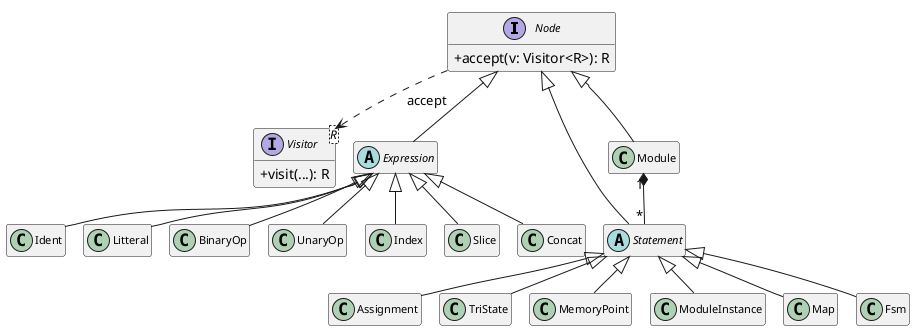
\includegraphics[width=0.95\textwidth]{ast-classes.png}

{\small Figure --- Diagramme de classes simplifi\'e de l'AST (g\'en\'er\'e avec PlantUML, source \texttt{ast-classes.puml}).}
\end{center}

\section*{Difficult\'es et r\'eussites}

La principale difficult\'e a \'et\'e de garantir que la grammaire reste \emph{r\'eellement} LL(1) apr\`es chaque ajout de r\`egle. Le v\'erificateur de conflits, \'ecrit avant la grammaire, s'est r\'ev\'el\'e d\'ecisif~: plusieurs ambigu\"it\'es sur les instances de modules et sur les FSM ont \'et\'e d\'etect\'ees avant m\^eme la premi\`ere ex\'ecution du parser. La r\'eussite principale est l'immuabilit\'e stricte de l'AST, qui rend les passes aval (typage, g\'en\'eration d'automates) triviales \`a para\-ll\'eliser et \`a tester.

\section*{Manuel utilisateur}

\textbf{Pr\'e-requis}~: JDK~21+, JUnit~4 et Hamcrest fournis dans \texttt{lib/}.

\textbf{Compiler et ex\'ecuter les tests du parser}~:
\begin{verbatim}
  cd parser/ll1
  javac -cp ../../lib/junit-4.13.2.jar:../../lib/hamcrest-core-1.3.jar \
        -d ../../bin $(find . -name "*.java") \
        $(find ../../tests/parser/ll1 -name "*.java")
  java -cp bin:../../lib/junit-4.13.2.jar:../../lib/hamcrest-core-1.3.jar \
       org.junit.runner.JUnitCore parser.ll1.SanityTest
\end{verbatim}

\textbf{Parser un fichier SHDL depuis le code}~:
\begin{verbatim}
  Parser p = new Parser(new Lexer(source));
  Module m = p.parseFrom();   // retourne l'AST racine
  m.accept(monVisiteur);      // passe aval au choix
\end{verbatim}

Le code source est publi\'e sur la branche \texttt{feature/skeleton-javafx}. Le bilan collectif de fin d'it\'eration se trouve dans \texttt{docs/sprint1/2026-04-13-bilan-sprint1.md}.

\end{document}
